\subsection*{Линейные модели}

Теперь, с этим набором знаний, наконец-то можно начать что-то творить. Сегодня мы остановимся на задаче регрессии ($\mathbb{Y} = \mathbb{R}$). Для понимания можно представить, что существует какая"=то неизвестная нам функция, которая идеально справляется с задачей предсказания, т.е. идеально описывает наши данные. В таком ключе, наша задача сводится к построению функции, которая будет как можно ближе к вышеописанной:
\begin{equation*}
a: \mathbb{X} \rightarrow \mathbb{Y}
\end{equation*}

Конечно, рассматривать все подряд функции бессмысленно и долго, поэтому обычно сначала фиксируют какое-то семейство функций, которое будет рассматриваться. Сегодня мы поговорим о семействе \textit{линейных моделей}, которое можно записать как:
\begin{equation*}
\mathcal{A} = \{a ~|~ a(x) = w_0 + w_1x_1 + \dots + w_dx_d\}~,~w_i \in \mathbb{R}
\end{equation*}

т.е. все такие модели $a$, которые можно представить в виде линейной комбинации с... А что это?

Значения $w$ называются \textit{весами} "--- это такие параметры модели, через подбор которых модель научится выдавать предсказания. Значение $w_0$ выделяют отдельно и называют \texttt{bias} (смещение). Как осуществляется подбор этих параметров "--- пока что чёрный ящик, о котором сейчас не стоит задумываться. Лишь скажем, что процесс подбора этих $w$ называется \textit{обучением модели}.

Значит, наша модель берёт все признаки, каждый домножает на какой"=то специально подбираемый коэффициент, суммирует все полученное, и на выходе получает величину, которая, хотелось бы, является предсказанием.

Мы знаем (а если не знаем, то теперь знаем), что линейную комбинацию можно записать в виде скалярного произведения векторов, которое в свою очередь выглядит так
\begin{equation*}
a(x) = w_0 + \langle w, x \rangle
\end{equation*}

Чтобы записать это совсем красиво, нам мешает $w_0$. Внесём следующее предположение: первый признак будет единичным (это легко сделать, просто нужно добавить к данным единичный столбец). Тогда $w_0$ станет весом этого признака, а вся запись получит вид:
\begin{equation*}
a(x) = \langle w, x \rangle
\end{equation*}

Только что мы вывели модель \textit{линейной регрессии}. Если мы построим линейную регрессию для одного признака, то получим 
\[
a(x) = w_1x_1 + w_0
\]

Вам это точно ничего не напоминает? Всё верно "--- это самое простое уравнение прямой. Отсюда вытекает следующая идея: геометрически идея линейной регрессии заключается в том, чтобы построить прямую (если признаков больше, то гиперплоскость), которая наилучшим образом описывает данные. Фразу <<наилучшим образом описывает данные>> можно наглядно увидеть на изображении ниже.

\begin{figure}[H]
\centering
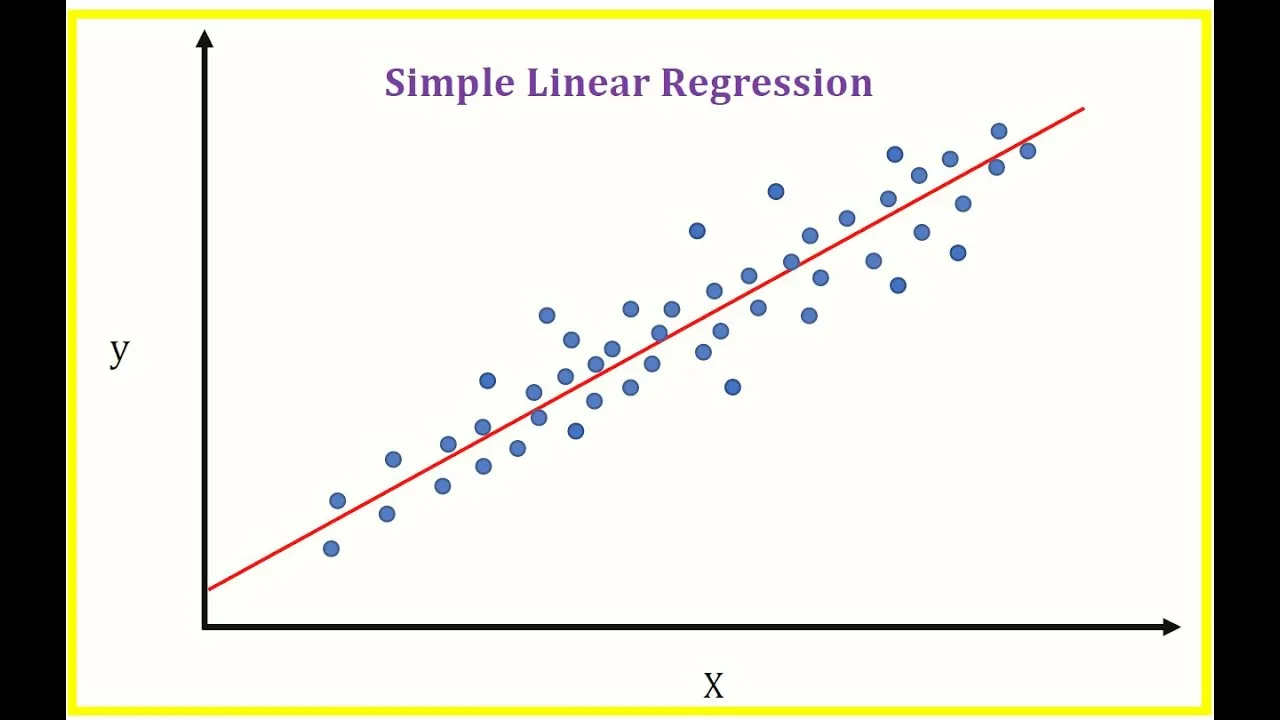
\includegraphics[width=0.8\linewidth]{media/linear_regression.png}
\end{figure}

Интуитивно то понятно, но как более формально определить наши наблюдения? Между каждой точкой и построенной прямой есть некоторое расстояние, и задача линейной регрессии в данном случае сводится к тому, чтобы построить прямую, у которой сумма всех таких расстояний наименьшая. Загвоздка лишь в том, что мы не можем заранее знать, когда эта сумма наименьшая.

Давайте также затронем ещё один момент, касающийся данных. Представим, что на изображении есть ещё одна точка, которая лежит очень далеко от всех остальных точек (и от прямой соответственно). Это означает, что этот объект содержит какое"=то аномальное значение признака или даже нескольких признаков (например, рост 200м). В общем, не суть "--- так или иначе у нас присутствует точка, которая в этом смысле сильно выделяется на фоне остальных. Такие объекты называются \textit{выбросами} (\texttt{outliers}).


Важно сразу определить серьёзный недостаток данной модели "--- мы делаем очень сильное предположение о том, что целевую переменную можно выразить с помощью линейной комбинации признаков, т.е. мы предполагаем, что между признаками и целевой переменной существует \textit{линейная зависимость}. На практике такое бывает крайне редко, но от этого ознакомление с этой моделью не становится бессмысленной "--- на её примере мы разобрали задачу регрессии, узнали про какие"=то веса и к чему в общем смысле сводится задача регрессии.

Также мы вскользь упомянули, что модель подбирает эти самые параметры до тех пор, пока не построит хорошую прямую. Но в какой момент мы поймём, что построенная прямая "--- достаточно хороша? Почему мы не можем просто построить пряммую, которая будет идеально предсказывать имеющиеся цены? По какому принципу обновляются веса? Об этом всём вы узнаете на следующем занятии.
